%% Based on a TeXnicCenter-Template by Tino Weinkauf.
%%%%%%%%%%%%%%%%%%%%%%%%%%%%%%%%%%%%%%%%%%%%%%%%%%%%%%%%%%%%%

%%%%%%%%%%%%%%%%%%%%%%%%%%%%%%%%%%%%%%%%%%%%%%%%%%%%%%%%%%%%%
%% HEADER
%%%%%%%%%%%%%%%%%%%%%%%%%%%%%%%%%%%%%%%%%%%%%%%%%%%%%%%%%%%%%
\documentclass[a4paper,twoside,10pt]{report}
% Alternative Options:
%	Paper Size: a4paper / a5paper / b5paper / letterpaper / legalpaper / executivepaper
% Duplex: oneside / twoside
% Base Font Size: 10pt / 11pt / 12pt


%% Language %%%%%%%%%%%%%%%%%%%%%%%%%%%%%%%%%%%%%%%%%%%%%%%%%
\usepackage[USenglish]{babel} %francais, polish, spanish, ...
\usepackage[T1]{fontenc}
\usepackage[ansinew]{inputenc}

\usepackage{lmodern} %Type1-font for non-english texts and characters


%% Packages for Graphics & Figures %%%%%%%%%%%%%%%%%%%%%%%%%%
\usepackage{graphicx} %%For loading graphic files
\usepackage{subfig} %%Subfigures inside a figure
%\usepackage{pst-all} %%PSTricks - not useable with pdfLaTeX

%% Please note:
%% Images can be included using \includegraphics{Dateiname}
%% resp. using the dialog in the Insert menu.
%% 
%% The mode "LaTeX => PDF" allows the following formats:
%%   .jpg  .png  .pdf  .mps
%% 
%% The modes "LaTeX => DVI", "LaTeX => PS" und "LaTeX => PS => PDF"
%% allow the following formats:
%%   .eps  .ps  .bmp  .pict  .pntg


%% Math Packages %%%%%%%%%%%%%%%%%%%%%%%%%%%%%%%%%%%%%%%%%%%%
\usepackage{amsmath}
\usepackage{amsthm}
\usepackage{amsfonts}


%% Line Spacing %%%%%%%%%%%%%%%%%%%%%%%%%%%%%%%%%%%%%%%%%%%%%
%\usepackage{setspace}
%\singlespacing        %% 1-spacing (default)
%\onehalfspacing       %% 1,5-spacing
%\doublespacing        %% 2-spacing


%% Other Packages %%%%%%%%%%%%%%%%%%%%%%%%%%%%%%%%%%%%%%%%%%%
%\usepackage{a4wide} %%Smaller margins = more text per page.
%\usepackage{fancyhdr} %%Fancy headings
%\usepackage{longtable} %%For tables, that exceed one page
\usepackage{color}

%%%%%%%%%%%%%%%%%%%%%%%%%%%%%%%%%%%%%%%%%%%%%%%%%%%%%%%%%%%%%
%% Remarks
%%%%%%%%%%%%%%%%%%%%%%%%%%%%%%%%%%%%%%%%%%%%%%%%%%%%%%%%%%%%%
%
% TODO:
% 1. Edit the used packages and their options (see above).
% 2. If you want, add a BibTeX-File to the project
%    (e.g., 'literature.bib').
% 3. Happy TeXing!
%
%%%%%%%%%%%%%%%%%%%%%%%%%%%%%%%%%%%%%%%%%%%%%%%%%%%%%%%%%%%%%

%%%%%%%%%%%%%%%%%%%%%%%%%%%%%%%%%%%%%%%%%%%%%%%%%%%%%%%%%%%%%
%% Options / Modifications
%%%%%%%%%%%%%%%%%%%%%%%%%%%%%%%%%%%%%%%%%%%%%%%%%%%%%%%%%%%%%

%\input{options} %You need a file 'options.tex' for this
%% ==> TeXnicCenter supplies some possible option files
%% ==> with its templates (File | New from Template...).



%%%%%%%%%%%%%%%%%%%%%%%%%%%%%%%%%%%%%%%%%%%%%%%%%%%%%%%%%%%%%
%% DOCUMENT
%%%%%%%%%%%%%%%%%%%%%%%%%%%%%%%%%%%%%%%%%%%%%%%%%%%%%%%%%%%%%
\begin{document}

\pagestyle{empty} %No headings for the first pages.


%% Title Page %%%%%%%%%%%%%%%%%%%%%%%%%%%%%%%%%%%%%%%%%%%%%%%
%% ==> Write your text here or include other files.

%% The simple version:
\title{Notes on modeling of growth-regulation interactions in the cAMP system}
\author{Martijn Wehrens}
%\date{} %%If commented, the current date is used.
\maketitle

%% The nice version:
%\input{titlepage} %%You need a file 'titlepage.tex' for this.
%% ==> TeXnicCenter supplies a possible titlepage file
%% ==> with its templates (File | New from Template...).


%% Inhaltsverzeichnis %%%%%%%%%%%%%%%%%%%%%%%%%%%%%%%%%%%%%%%
%\tableofcontents %Table of contents
\cleardoublepage %The first chapter should start on an odd page.

\pagestyle{plain} %Now display headings: headings / fancy / ...



%% Chapters %%%%%%%%%%%%%%%%%%%%%%%%%%%%%%%%%%%%%%%%%%%%%%%%%
%% ==> Write your text here or include other files.

%\input{intro} %You need a file 'intro.tex' for this.


%%%%%%%%%%%%%%%%%%%%%%%%%%%%%%%%%%%%%%%%%%%%%%%%%%%%%%%%%%%%%
%% ==> Some hints are following:

%\chapter{Some small hints}\label{hints}

%\section{German Umlauts and other Language Specific Characters}\label{umlauts}

\chapter{Modeling the noise transmission}

\section{Ornstein-Uhlenbeck fluctuations model}

\subsection{The model}

In these notes I discuss a model which models how noise originates and transmits from and between observables respectively. I will discuss the model proposed by Philippe Nghe in the work by Kiviet et al. \cite{Kiviet2014}, and also possible extensions and modifications to this model.

Parameters that are considered in general are the number of enzymes ($E$), the rate at which these enzymes are made ($p$), and the growth rate of the cell ($\lambda$). Generally, enzymes only disappear by dilution due to growth. Furthermore, there are noise sources, which add noise to these parameters. Depending on how they are implemented these source appear as $N_M$, $N_\lambda$ and $N_p$ or $\Gamma_M$, $\Gamma_\lambda$ and $\Gamma_p$, the subscripts indicate to which parameter the noise source adds noise.

The goal of this model is to interpret the cross-correlations between $\lambda$, $E$ and $p$ (usually $R_{E,\lambda}(\tau)$, $R_{p,\lambda}(\tau)$), that are obtained from experimental data.

\subsection{Implicit noise equations}


\begin{figure}
	\centering
	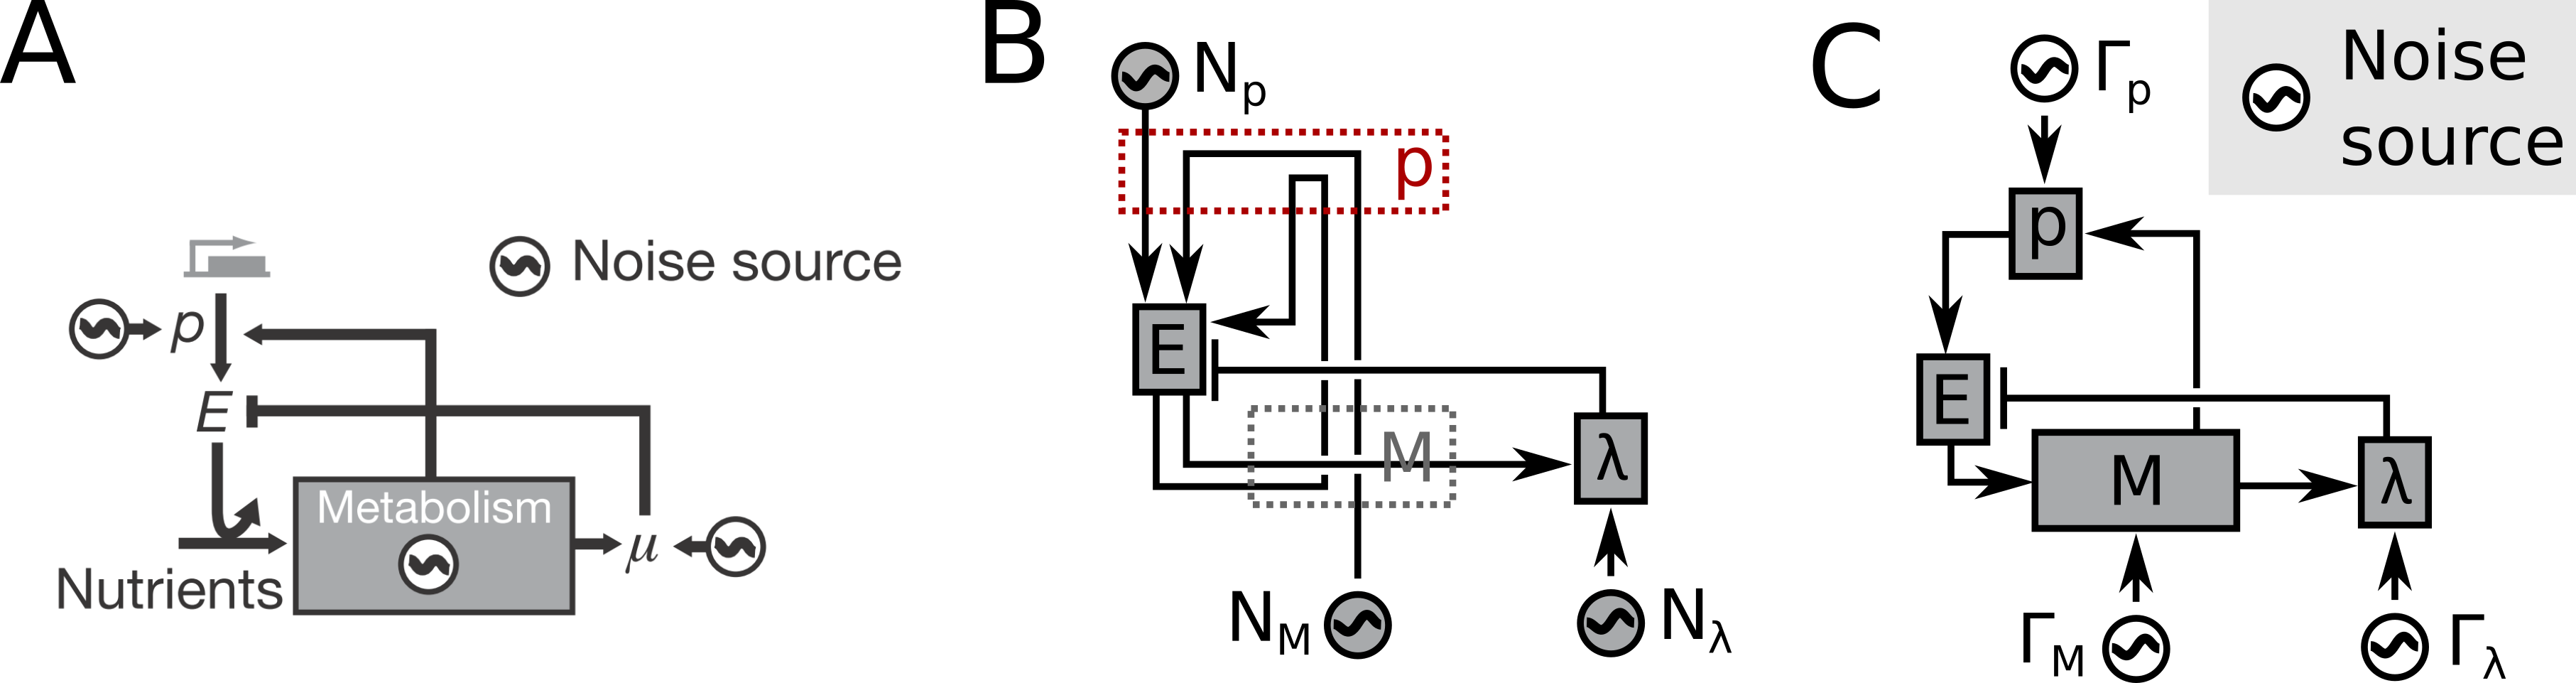
\includegraphics[width=0.9\textwidth]{./drawings_png/model_nghe_v2.png}
	\caption{ 
		(A) Original diagram as printed in Kiviet et al. \cite{Kiviet2014}.
		(B) More technical diagram stating the relations between parameters of interest (gray boxes), and noise sources $N_P$, $N_M$, and $N_\lambda$. Arrows indicate how ODEs or functions that describe the parameters of interest are coupled. 
		Arrows that go trough the red dashed box correspond to terms that not only couple the two parameters connected by the arrow, but also make up the parameter $p$ (see also main text).
		Arrows that go through the grey box are arrows which are thought to be biologically connected to the metabolism.
		(C) An alternative version of the model with more parameters modelled explicitly. Noise sources are printed white in this diagram since they are not described by separate ODEs, which was the case in Kiviet et al. \cite{Kiviet2014}. 
	}
	\label{fig:modeldrawing}
\end{figure}

A straight forward way to model a system with these parameters, is writing down an ordinary differential equation (ODE) for each parameter involved. 
%
The Nghe model takes a somewhat different approach (it is more concise), which will be discussed later.
%
The ODEs below relate to the cartoon in Fig. \ref{fig:modeldrawing}.C
and describe the dynamics per parameter:
%
\begin{align}
\label{myfirstequation}
\dot{M} = & - \frac{(M-M_0)}{\tau}  \nonumber \\ 
          & + c_M \cdot \Gamma_M  \nonumber \\ % (1-T_{M\leftarrow E})
          & + T_{M\leftarrow E} \cdot c_M \cdot (\frac{E}{E_0} - 1)  
\end{align}
% deltaMetabolism = -(metabolismValues(end)-parameters.metabolism0) * 1/parameters.dampingTimeMetabolism + ... % damping; 1 is the equilibrium value
% (1-parameters.transmissionEnzymeMetabolism) * ((rand()-.5)*2) * parameters.noiseSizeMetabolism + ...                              % white noise component
% parameters.transmissionEnzymeMetabolism * (enzymeValues(end)/parameters.enzymeTarget-.5) * parameters.noiseSizeMetabolism;             % noise component due enzyme
%
%
\begin{align}
	\dot{\lambda} = & -\frac{(\lambda - \lambda_0 )}{\tau_\lambda} \nonumber \\ 
 			& + c_\lambda \cdot \Gamma_\lambda \nonumber \\  %  (1-T_{\lambda\leftarrow M}) \cdot
			& +    T_{\lambda\leftarrow\ M} \cdot c_\lambda \cdot (\frac{M}{M_0}-1) 
\end{align}
%
\begin{align}
\label{mythirdequation}
\dot{P} = & - \frac{(P-P_0)}{\tau_P} \nonumber \\ 
		 & + c_\lambda \cdot \Gamma_\lambda \nonumber \\ 
         & + T_{P\leftarrow M} \cdot c_P \cdot (\frac{M}{M_0}-1)  \nonumber \\ 
         & + R_{P\leftarrow M} \cdot c_P \cdot (\frac{M}{M_0}-1)
\end{align}
%
\begin{align}
\label{mylastequation}
\dot{E} = P - \lambda E
\end{align}
%
Where $M$ describes the state of the metabolism, $\lambda$ is the growth rate, $P$ is the production rate, $E$ is the amount of enzyme, $\tau$ is a dampening term ($X_0$ is the equilibrium value), $T_{X \leftarrow Y}$ is the noise transmission constant from $X$ towards $Y$, $c_X$ is a constant that sets the size of the fluctuations, $\Gamma_X$ is a white noise source.
$R_{X \leftarrow Y}$ indicates a regulatory interaction, an addition to the model by me, but this notation is currently just cosmetical, as $T_\text{effective}=T+R$.
%
This model assumes all parameters have an average value from which fluctuations deviate, but always return. Hence the dampening terms.
With respect to transmission, I furthermore rescale the absolute value of the noise to be comparable to the target noise (hence the $M_0^{-1}$ and $c_X$ terms in combination with the $T_{X\leftarrow Y}$ term).

This is similar to the model that Philipe Nghe had in Kiviet et al. \cite{Kiviet2014}, which was inspired by Dunlop et al. \cite{Dunlop2008} (see supplement of that manuscript for a description of the Dunlop model).
%
A difference between my equations, the Nghe equations and the Dunlop equations lies in the dampening terms (those containing $\tau$, $\beta$ or $\mu_E$). In my model noise is effected through the ODE, and dampening occurs on the parameter of interest. In Dunlop et al., there are two dampening terms, one specifically dampening the noise and a second term dampening the parameters of interest. It seems also Nghe takes the latter approach, dampening being effected through the $(-\beta_X \cdot N_X)$ term and the $\mu_E$ parameter (see later for a more involved discussion on these parameters).

The correlations between these equations can be found by linearizing them, writing the correlations in Fourier space, and back-transforming them using residue integration techniques. 
This document currently does not fully explores this, but this will partially be discussed later.
First, a comparison with the Nghe model is made.

\section{Separate noise equations}

Both Nghe and Dunlop define separate ODEs for the noise terms:
%
\begin{align}
\label{eq:generalgillespienoise}
\dot{N}_X = \sqrt{C_X} \cdot \Gamma_X - N_X/\tau
,
\end{align}
%
though their notation might be slightly different (I used Daniel Gillespie's notation \cite{Gillespie1996}; a capital C is used here to follow Gillespie's square root notation, $\sqrt{C_X}=c_x$).
With for our case $X$ equaling $\lambda$, $M$ or $P$. Note that $\tau^{-1}=\beta$ ($\beta$ is used in Nghe and Dunlop).

Not so relevant for our case, but noteworthy, is that in the Dunlop model, which models a completely different process than the one described here \cite{Dunlop2008}, the \textit{solutions} of the ODEs describing the noise are plugged into the ODEs describing the protein dynamics. This leads to an additional memory effect.
%
That is:
%
\begin{align}
\label{dunlopgeneralequation}
\dot{X} = & N_X  + F(X) + X/\tau
,
\end{align}
%
with $F(X)$ some arbitrary function of $X$. 
Note that the $N_X$ function also contains a $\tau$ term (see Eq. \ref{eq:generalgillespienoise}), which is effectively integrated, thus leading to effects of the fluctuations much longer timescales than $\tau$. 
This effect is (partially) countered by the third term in Eq. \ref{dunlopgeneralequation}, which also contains the $\tau$ term.

\section{Nghe model}

As mentioned, the Nghe model takes a different approach. 
The formulae that follow correspond to Fig. \ref{fig:modeldrawing}.B (Fig. \ref{fig:modeldrawing}.A contains a more polished version of that cartoon that was published in Kiviet et al.).
The starting point,
%
\begin{align}
\label{eq:Nghe1}
\dot{E} = P - \lambda E
,
\end{align}
%
is the same in my model, but after linearization (defined as $X=X_0+\delta X$) this leads to only one ODE (see written notes from 28.9.2016 for explicit linearization):
%
\begin{align}
\label{eq:ODEElinearized}
\frac{ \delta{\dot{E}} }{E_0 \mu_0} 
+ \frac{\delta E}{E_0} 
%& = 
%\left[
% T_{E \leftarrow E} \frac{\delta E}{E_0} + T_{E \leftarrow G} N_G + N_E 
% \right]
% + T_{E \leftarrow \mu} \frac{\delta \mu}{\mu_0} \nonumber \\
& =
\frac{\delta p}{E_0 \mu_0} + T_{E \leftarrow \mu} \frac{\delta \mu}{\mu_0}
.
\end{align}
%
Noise terms are introduced with ODEs that are also shown above in Eq. \ref{eq:generalgillespienoise}.
 Additionally, two functions are defined for $p$ and $\lambda$. These are not ODEs, as the effects on these parameters are thought to happen on fast timescales. The parameters are however linearized (and thus written as $\delta X$). The equation
%
\begin{align}
\label{eq:Nghe3}
\frac{\delta\mu}{\mu_0} = T_{\mu \leftarrow E} \frac{\delta E}{E_0} + T_{\mu \leftarrow G} N_G + N_\mu
\end{align}
%
simply defines the evolution of $\delta \mu$.
There is also an equation for $\delta p$
%
\begin{align}
\label{eq:Nghe4}
\frac{\delta{p}}{E_0 \mu_0} = T_{E \leftarrow E} \frac{\delta E}{E_0} + T_{E \leftarrow G} N_G + N_E
,
\end{align}
%
which plays a bit more complicated role.
It is defined using terms that pertain to E, like $T_{E \leftarrow G}$, such that it can be directly plugged into Eq. \ref{eq:ODEElinearized}. 
Indeed, plugging Eq. \ref{eq:Nghe4} into Eq. \ref{eq:ODEElinearized} leads to equation:
%
\begin{align}
\label{eq:Nghe5}
\frac{ \delta{\dot{E}} }{E_0 \mu_0} 
+ \frac{\delta E}{E_0} 
& = 
\left[
 T_{E \leftarrow E} \frac{\delta E}{E_0} + T_{E \leftarrow G} N_G + N_E 
 \right]
 + T_{E \leftarrow \mu} \frac{\delta \mu}{\mu_0} 
\end{align}
%
which corresponds to equation 5 in the Kiviet et al. \cite{Kiviet2014} manuscript.
I say it is a bit complicated, since Eq. \ref{eq:Nghe4} has no role in the model (we could also just have defined Eq. \ref{eq:Nghe5} immediately), except that it shows us which part of the model can be interpreted as being the production rate.
This is also the reason why $p$ is depicted as a red dashed box in Fig. \ref{fig:modeldrawing}.

%
%{\color{red}
%There are currently a few things unclear about Eq. \ref{eq:Nghe3} and Eq. \ref{eq:Nghe4} (respectively Eq. 3 and 4 in the Kiviet et al. manuscript):
%\begin{itemize}
%\item It seems that the transmission terms $T_{X\leftarrow Y}$ state how the parameter of interest ($X$) is affected by another parameter of interest ($Y$), however, for this to be true, the left-hand side parameter should match the first parameter in the subscript of $T$. E.g. how can a $T_{E\leftarrow G}$ term appear in the equation for $\delta p$ and moreover, what does the term $T_{E \leftarrow E}$ mean?
%\item It is not clear to me how these formulae relate to the diagram that was drawn (see Fig. \ref{fig:modeldrawing}). Why is E directly effecting $\mu$? Should there not also be a metabolism term $G$ or $\delta G$? Also why does the formula for $\delta p$ contain transmission from $E$ (assuming $T_{E\leftarrow E}$ was a type and should have been $T_{p\leftarrow E}$)? Why does the formula for $\delta p$ contain a noise term for E (ie. $N_E$)?
%\item These are not ODEs (which would seem more natural to me), probably this is intended this way, and the relationship between the parameters is defined as such. (And could be derived from ODEs.)    
%\end{itemize}
%%I am currently not sure how these equations relate to my own equations, as subscripts in Eq. \ref{eq:Nghe4} seem inconsistent with the fact that transmission should be towards $P$ (e.g. what is $T_{E\leftarrow E}$?).
%}
%
%In any case, given that noise and other parameters are related in terms of parameters (not derivatives), the following formulae are probably underlying the Nghe model:
%
%\begin{align}
%\dot{M} = & \dot{N}_M  \nonumber \\ 
%& + T_{M\leftarrow E} \cdot c_M \cdot (\frac{E}{E_0} - 1)  
%\end{align}
%
%\begin{align}
%\dot{\lambda} = & \dot{N}_\lambda \nonumber \\ 
%& +    T_{\lambda \leftarrow M} \cdot c_\lambda \cdot (\frac{M}{M_0}-1) 
%\end{align}
%
%\begin{align}
%\dot{P} = & \dot{N}_P \nonumber \\ 
%& + T_{P\leftarrow M} \cdot c_P \cdot (\frac{M}{M_0}-1)  \nonumber \\ 
%& + R_{P\leftarrow M} \cdot c_P \cdot (\frac{M}{M_0}-1)
%\end{align}
%
%Where the normalizations by $X_0$ were left out again.

Note however, that this results in the absence of dampening terms on the parameters $X$ themselves, which leads to non-steady state behavior of the parameters.
The term $X/\tau$ could be added to each of the equations to resolve this issue; the term $-N_X/\tau$ from the noise ODEs could then be dropped.
{\color{red}Note that a $\mu_E$ term appears eventually in Nghe's equations, which might play the role of a second dampening term.}



%%%%%%%%%%%%%%

\section{Obtaining the cross correlations}

{\color{red}TODO: Process below such that it correctly handles Philippe's and my model (text above has been updated after phone call w. PN). Discuss w. ST/others whether and how to expand model.}

\subsection{Obtaining solutions in Fourier space}

How do we get the cross correlations? A way to define correlations is\footnote{From Wikipedia, https://en.wikipedia.org/wiki/Cross-correlation and Weisstein, Eric W. "Cross-Correlation Theorem." From MathWorld--A Wolfram Web Resource. http://mathworld.wolfram.com/Cross-CorrelationTheorem.html}:

\begin{align}
R_{f,g}(\tau) = f \star g = \int_{\tau=\infty}^{\infty} {\bar f(\tau) g(t+\tau) \delta \tau}
\end{align}

With the $\bar{f}$ denoting the complex conjugate. This is equal to the convolution of $f^*(-t)$ and $g(t)$, 

\begin{align}
f \star g = f*(-t) * g
.
\end{align}

It can be derived that:

\begin{align}
\mathcal{F} (f \star g) = \overline{\mathcal{F} (f)} \mathcal{F}(g)
.
\end{align}

This property can be exploited to find the cross correlation that we are interested in:

\begin{align}
R_{\mu,E}(\tau) = \mathcal{F}^{-1} \left( \overline{\mathcal{F} (\mu)} \mathcal{F}(E) \right)
.
\end{align}

First we find the solutions to the ODEs in Fourier space:

\begin{align}
\label{ODEEFourier}
\mathcal{F} \left( \dot{E} \right) = & \mathcal{F} \left( P - \lambda E \right) \nonumber \\
%
i\omega \tilde{E} = & \tilde{P} - \tilde{\lambda} \tilde{E}
\end{align}

\begin{align}
 \tilde{E} = & \frac{1}{i\omega+\tilde{\lambda}} \tilde{P} 
\end{align}

For Eq. \ref{eq:generalgillespienoise} the solution in Fourier space is:

\begin{align}
\tilde{N}_X = \frac{\sqrt{c_x}}{i\omega - 1/\tau} \tilde{\Gamma}_x
\end{align}

which however will not be directly used to solve Eq. \ref{myfirstequation}-\ref{mylastequation}. With regard to  Eq. \ref{myfirstequation}-\ref{mythirdequation}, the solutions in general terms can be found from taking the Fourier transform:

\begin{align}
i \omega \tilde{X} = - \frac{\tilde{X}-X_0}{\tau_X} + c_X \tilde{\Gamma}_X + T_{X \leftarrow Y} c_X (\frac{\tilde{Y}}{X_0} - 1)
\end{align}

which, solving for $X$ gives:

\begin{align}
\label{solutionXFourier}
\tilde{X} = \left( i \omega + \frac{1}{\tau_X} \right)^{-1} \left( \frac{X_0}{\tau_X} + c_X \tilde{\Gamma}_X + T_{X \leftarrow Y} c_X (\frac{\tilde{Y}}{Y_0} - 1) \right)
,
\end{align}

$X$ being either $\lambda$, $M$ or $P$.
%
The solution for $E$ in Fourier space (i.e. to Eq. \ref{mylastequation}) without $P$ or $\lambda$ terms is very involved. This can be seen by plugging Eq. \ref{solutionXFourier} into Eq. \ref{ODEEFourier}, which results in:

\begin{align}
\label{ODEEFourierExpanded}
i\omega \tilde{E} = & 
%P
\left( i \omega + \frac{1}{\tau_P} \right)^{-1} \left( \frac{P_0}{\tau_P} + c_P \tilde{\Gamma}_P + T_{P \leftarrow M} c_P (\frac{\tilde{M}}{M_0} - 1) \right)
     \nonumber \\
    & -
    % lambda
    \left( i \omega + \frac{1}{\tau_\lambda} \right)^{-1} \left( \frac{\lambda_0}{\tau_\lambda} + c_\lambda \tilde{\Gamma}_\lambda + T_{\lambda \leftarrow M} c_\lambda (\frac{\tilde{M}}{M_0} - 1) \right)
     \tilde{E}
\end{align}
Where M is defined as:

\begin{align}
\label{solutionForM}
\tilde{M} = \left( i \omega + \frac{1}{\tau_M} \right)^{-1} \left( \frac{M_0}{\tau_M} + c_M \tilde{\Gamma}_M + T_{M \leftarrow E} c_M (\frac{\tilde{E}}{E_0} - 1) \right)
\end{align}

Plugging Eq. \ref{solutionForM} into Eq. \ref{ODEEFourierExpanded} results in an equation where the only time-dependent parameter is E.
Solving that formula for E gives a very involved formula, which is not displayed here.

\subsection{Actually getting the cross-correlations}

As Dunlop et al. point out, we are now looking at the expectation values of the correlation functions (since we're talking about noise), so in general terms:

\begin{align}
\left< R_{X,Y}(\tau)\right > = 
\left< \mathcal{F}^{-1} \left[ \overline{\mathcal{F} (X)} \mathcal{F}(Y) \right] \right>
\end{align}

\section{Towbin model}

\begin{align}
\text{F}(\text{x})\text{=}\frac{\text{K1}}{\text{K1}+x}
\end{align}

\begin{align}
\frac{\partial x(t)}{\partial t}=\beta  C(t) \text{F}(x)-\frac{\gamma  x \left(1-C(t)\right)}{\text{K2}+x}
\end{align}
Set to zero to find steady state concentration.

Here, in the first term on rhs, $\beta$ is the efficiency at which the carbon sector (C) converts sugars into metabolites (x). F(x) describes immediate feedback by x. External sugar concentration is assumed constant, and import + conversion directly dependent C, and thus there is no term "s" in this formulae.
The 2nd time rhs describes the consumption of x, which results in growth. $(1-C[t]) = R$, or the ribosomal sector. $\Gamma$ is some efficiency factor, $x/(x+K2)$ describes reaction kinetics of conversion of x to growth (Michaelis-Menten kinetics aka Hill). 
We propose x can actually be regarded as in steady state, as the time scales of this reaction are much faster than any other, hence $dX(t),t = 0$. 

\begin{align}
\frac{\partial C(t)}{\partial t}=f(x) \mu (t)-C \mu =\mu (t) \left(f(x)-C(t)\right);
\end{align}

Here, 1st term rhs describes that how many proteins are produced depends on the growth rate of the cell (Hwa - but generalized from constant). The 2nd term simply describes dilution.

\begin{align}
\mu (t)=\frac{\alpha  \left(\gamma  x \left(1-c_t\right)\right)}{\text{K2}+x}
\end{align}

\section{Notes}

Note that Philippe Nghe's scripts can be found at:

\begin{verbatim}
    \\storage01\data\AMOLF\groups\tans-group\Former-Users\
    Nghe\Noise_Growth\matlab3
\end{verbatim}


%% <== End of hints
%%%%%%%%%%%%%%%%%%%%%%%%%%%%%%%%%%%%%%%%%%%%%%%%%%%%%%%%%%%%%



%%%%%%%%%%%%%%%%%%%%%%%%%%%%%%%%%%%%%%%%%%%%%%%%%%%%%%%%%%%%%
%% BIBLIOGRAPHY AND OTHER LISTS
%%%%%%%%%%%%%%%%%%%%%%%%%%%%%%%%%%%%%%%%%%%%%%%%%%%%%%%%%%%%%
%% A small distance to the other stuff in the table of contents (toc)
\addtocontents{toc}{\protect\vspace*{\baselineskip}}

%% The Bibliography
%% ==> You need a file 'literature.bib' for this.
%% ==> You need to run BibTeX for this (Project | Properties... | Uses BibTeX)
%\addcontentsline{toc}{chapter}{Bibliography} %'Bibliography' into toc
%\nocite{*} %Even non-cited BibTeX-Entries will be shown.
%\bibliographystyle{alpha} %Style of Bibliography: plain / apalike / amsalpha / ...
\bibliography{./../../library} %You need a file 'literature.bib' for this.
\bibliographystyle{plain}

%%% The List of Figures
%\clearpage
%\addcontentsline{toc}{chapter}{List of Figures}
%\listoffigures
%
%%% The List of Tables
%\clearpage
%\addcontentsline{toc}{chapter}{List of Tables}
%\listoftables
%%}

%%%%%%%%%%%%%%%%%%%%%%%%%%%%%%%%%%%%%%%%%%%%%%%%%%%%%%%%%%%%%
%% APPENDICES
%%%%%%%%%%%%%%%%%%%%%%%%%%%%%%%%%%%%%%%%%%%%%%%%%%%%%%%%%%%%%
\appendix
%% ==> Write your text here or include other files.

%\input{FileName} %You need a file 'FileName.tex' for this.


\end{document}

